\textbf{ShoppingList}

ShoppingList er oprettet som en ViewModel. Den egentlige model til ShoppingList er PurchaseProducts, som implementeres gennem ObservableCollection<T> som ShoppingList arver fra.\\
Der kan redigeres i shoppinglisten via \gls{KA} midterpanels knapper, som er bundet til ShoppingLists commands(RelayCommand~\cite{RelayC}). Disse commands kontrollerer desuden hvornår knapperne i GUI'en er disabled.\\
ShoppingList er placeret i Business Logic Layer da denne desuden har nogle funktionens kald som kaldes fra ProductButtonControl. Disse funktioner har eksempelvis til ansvar at kontrollere om et produkt, som ønskes tilføjet, allerede er på listen og i såfald inkrementeret antal istedet for at tilføje igen. 

\begin{figure}[H]
	\centering
	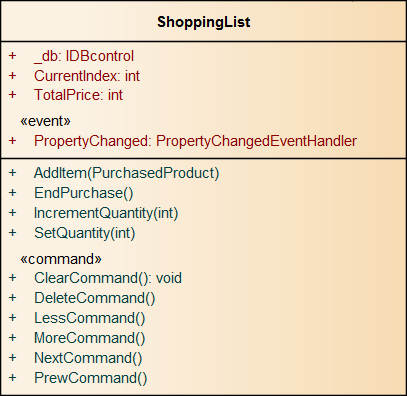
\includegraphics[width=60mm]{Systemdesign/Frontend/BLL/Pics/ShoppingList}
	\caption{ShoppingList}
	\label{fig:ShoppingList}
\end{figure}

\bigskip